\documentclass[12pt]{article}
\usepackage{parskip}
\usepackage{amsmath}
\usepackage{pdfpages}
\usepackage{listings}
\usepackage{color}
\usepackage[margin=.6in]{geometry}

\definecolor{dkgreen}{rgb}{0,0.6,0}
\definecolor{gray}{rgb}{0.5,0.5,0.5}
\definecolor{mauve}{rgb}{0.58,0,0.82}

\lstset{frame=tb,
  language=C++,
  aboveskip=3mm,
  belowskip=3mm,
  showstringspaces=false,
  columns=flexible,
  basicstyle={\small\ttfamily},
  numbers=none,
  numberstyle=\tiny\color{gray},
  keywordstyle=\color{blue},
  commentstyle=\color{dkgreen},
  stringstyle=\color{mauve},
  breaklines=true,
  breakatwhitespace=true,
  tabsize=3
}
\begin{document}
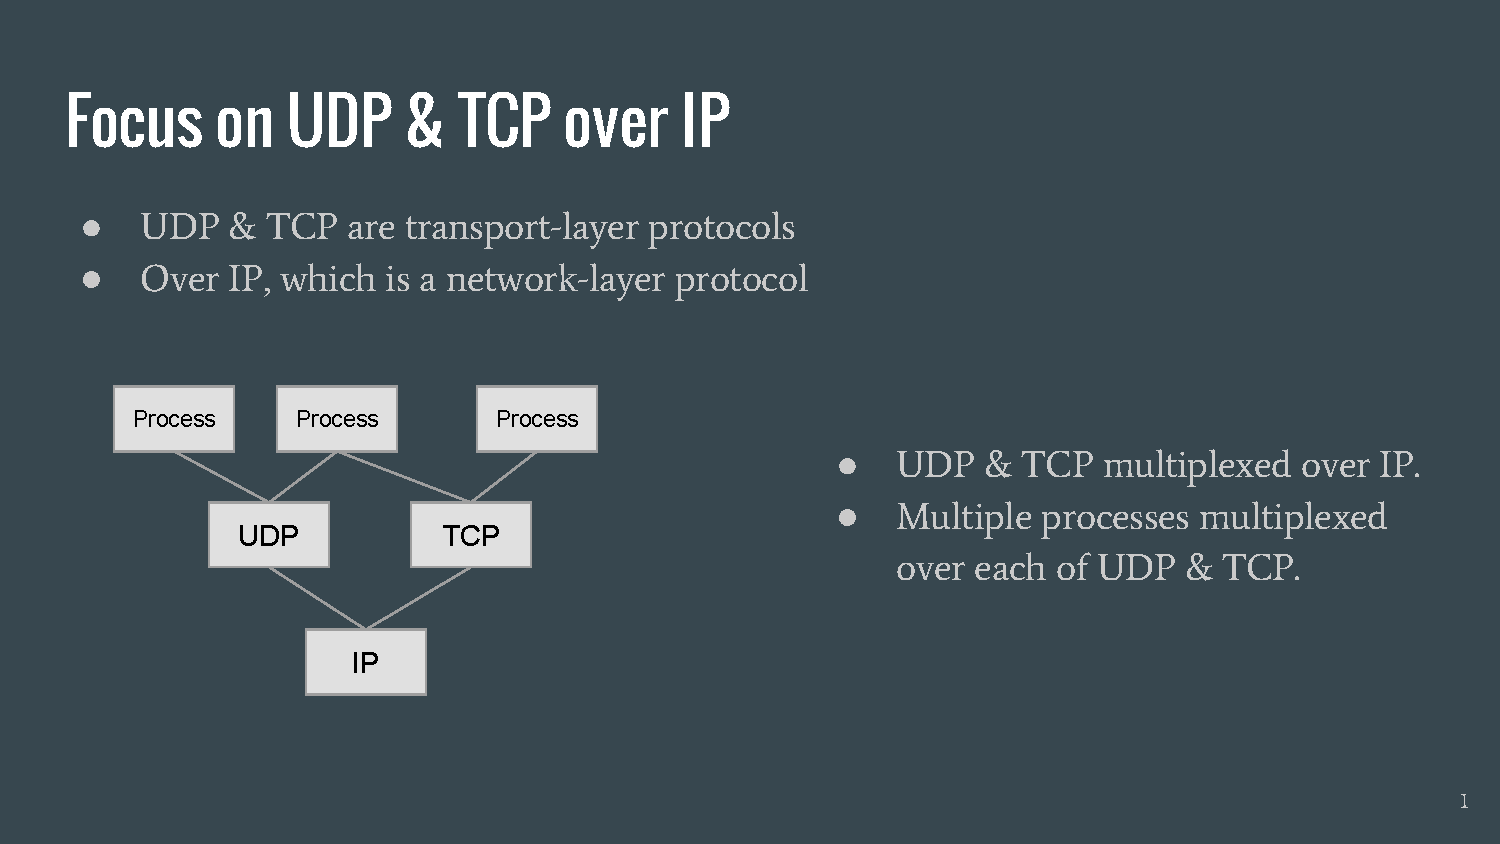
\includepdf[page=1-3]{slides.pdf}
\section{5 Tuple} % (fold)
\label{sec:5_tuple}
We can understand the flow of the packet through your system by looking at the 5-tuple. 
\begin{itemize}
	\item source ip address
	\item source port
	\item destination ip address
	\item destination port
	\item protocol
\end{itemize}
		
% section 5_tuple (end)
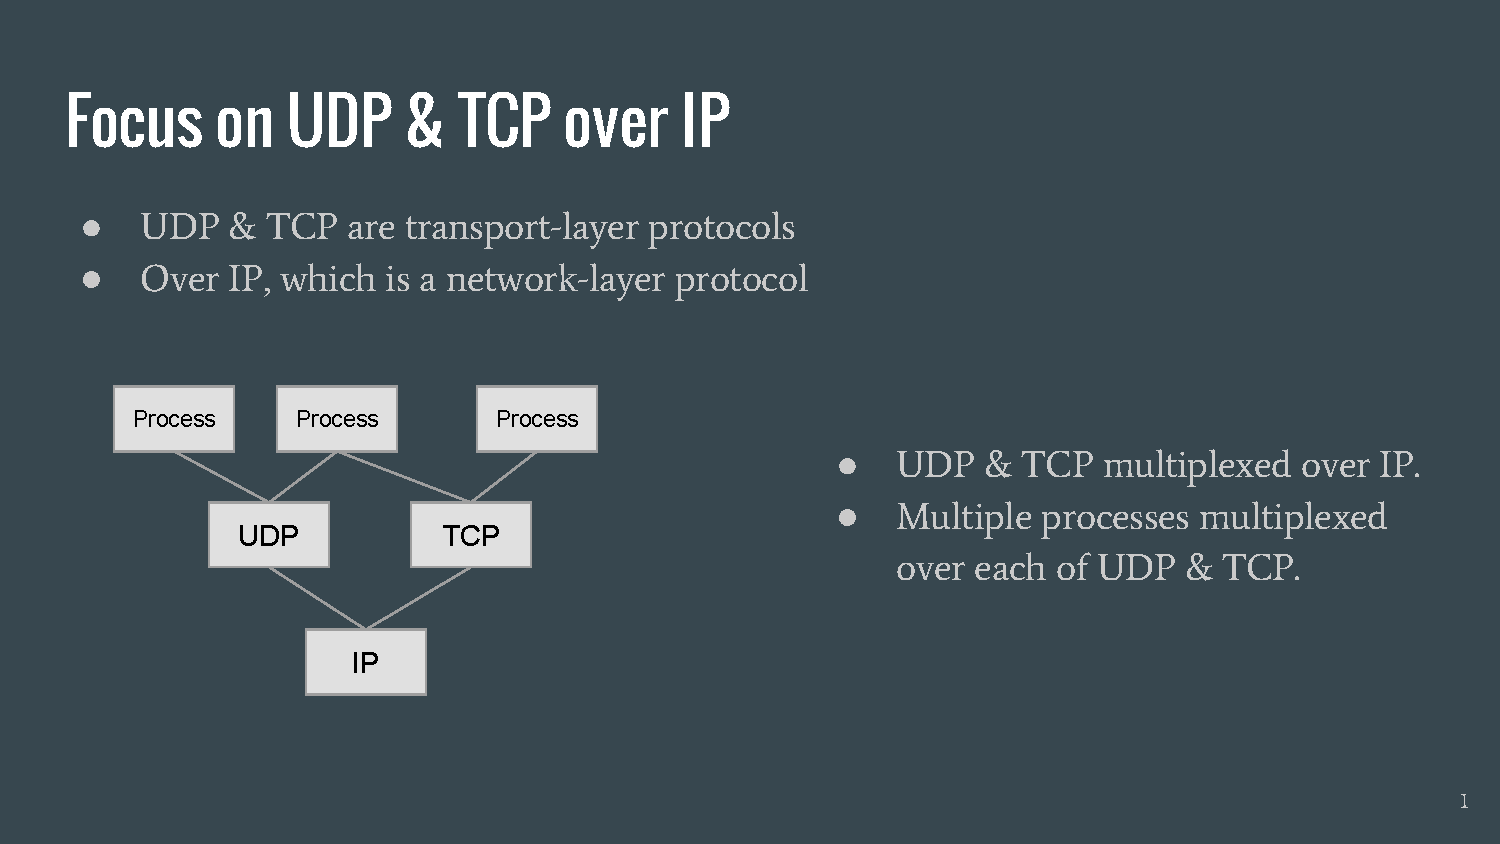
\includepdf[page=4]{slides.pdf}
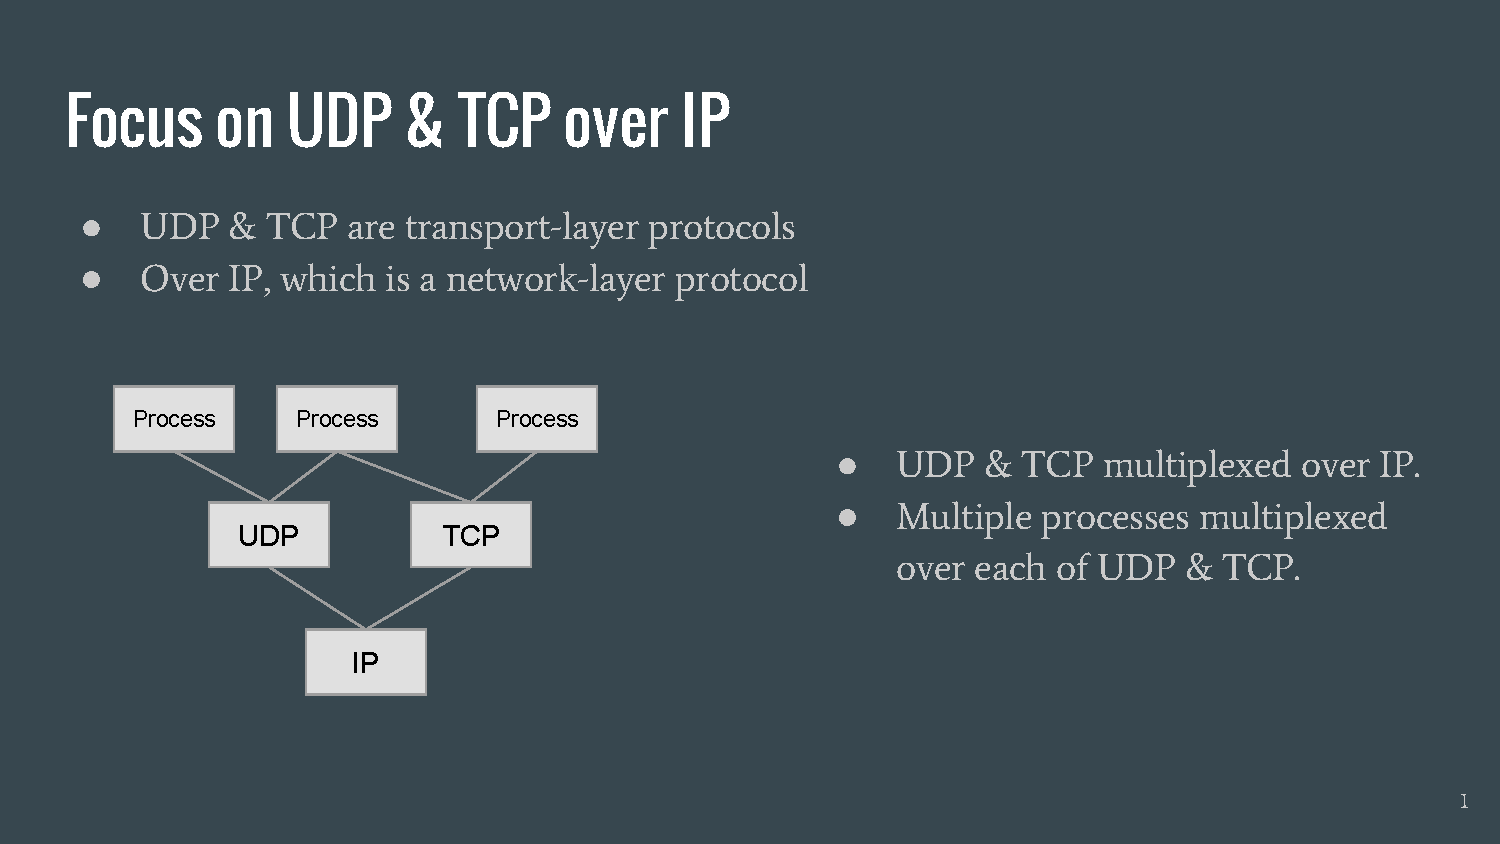
\includepdf[page=5]{slides.pdf}
\section{Socket API} % (fold)
\label{sec:socket_api}
Here a the 9 basic socket commands.

Here is a UDP example:
You have multiple identities association with ip so you can just chose one or use all of them. 

Checkout \texttt{man 7 ip} for more information.


\begin{lstlisting}
struct in_addr // this is a struct for internet addresses, it is just a uint32

int sockfd = -1
if(sockfd == socket(AF_INET, SOCK_DGRAM, 0) < 0) { // see man socket to learn how this function works
	//shit done borked
	return -1
}

struct sockaddr_in server
server.sin_port = 0 // some ports have specific privileges and such, 0 allows the OS to pick the port
server.sin_port_family = AF_INET 
if(bind(sockfd, (struct aockaddr_in *)&server, sizeof(struct socaddr_in)) < 0) { // see man bind
	//what did you do wrong
	return -1
}

if(getsockname(sockfd, (struct sockaddr) &server, sizeof(struct socaddr_in)) < 0){ //man getsockname to get the socket address
	//seriously how did you fuck this up
	return -1
}

print(inet_ntoa(server.sin_addr))
print(ntohs(server, sin_port))

//make sure you put that buffer length thing properly (see buffer overflow attacks, hee hee)
//this is blocking which is why you have to check the reclen, might actually need a loop here
if(reclen = recfrom(sockfd, buffer, bufferlength-1, 0, (struct socketaddr *) &client, sizeof(struct sockaddr_in)) < 0) { // man recvfrom
	//layyyyyme
	return -1;
}

print(inet_ntoa(client.sin_addr))
print(ntohs(client, sin_port))

//dont forget to close your shit
close(sockfd)


//To get the address you want, in a separte program
getifaddrs
//avoid memory leaks
freeifaddrs

struct ifaddrs *ifa //this is a linked list
if(getifaddrs(&ifa) < 0){
	return -1
}

for(struct ifaddrs *1 ifa; i != NULL; i = i->ifa_next) {
	if(i->ifa_addr == NULL) continue 

	//add address to list of available addresses that the user can use
}


\end{lstlisting}


We need to watch for big/little endian cause OSs are separate from networks. We have a call in in\_addr that will fix its shit for us. 

CHECK YOUR RETURN VALUES FUCKER!!! This shit sucks to debug. LARA I'M LOOKING AT YOU, IF YOU FUCK THIS UP I WILL KILL YOU.

You might need to compile with a flag -D\_BSD\_SOURCE

TCP works very similar to the above UDP example except that it is connection oriented. So instead of just checking how much data was received you must listen, accept, and receive. After you accept it locks the server from accepting more connections. All the same checks and such must happen.  
% section socket_api (end)

Helpful commands:
\begin{itemize}
	\item man all the pages
	\item netstat
\end{itemize}



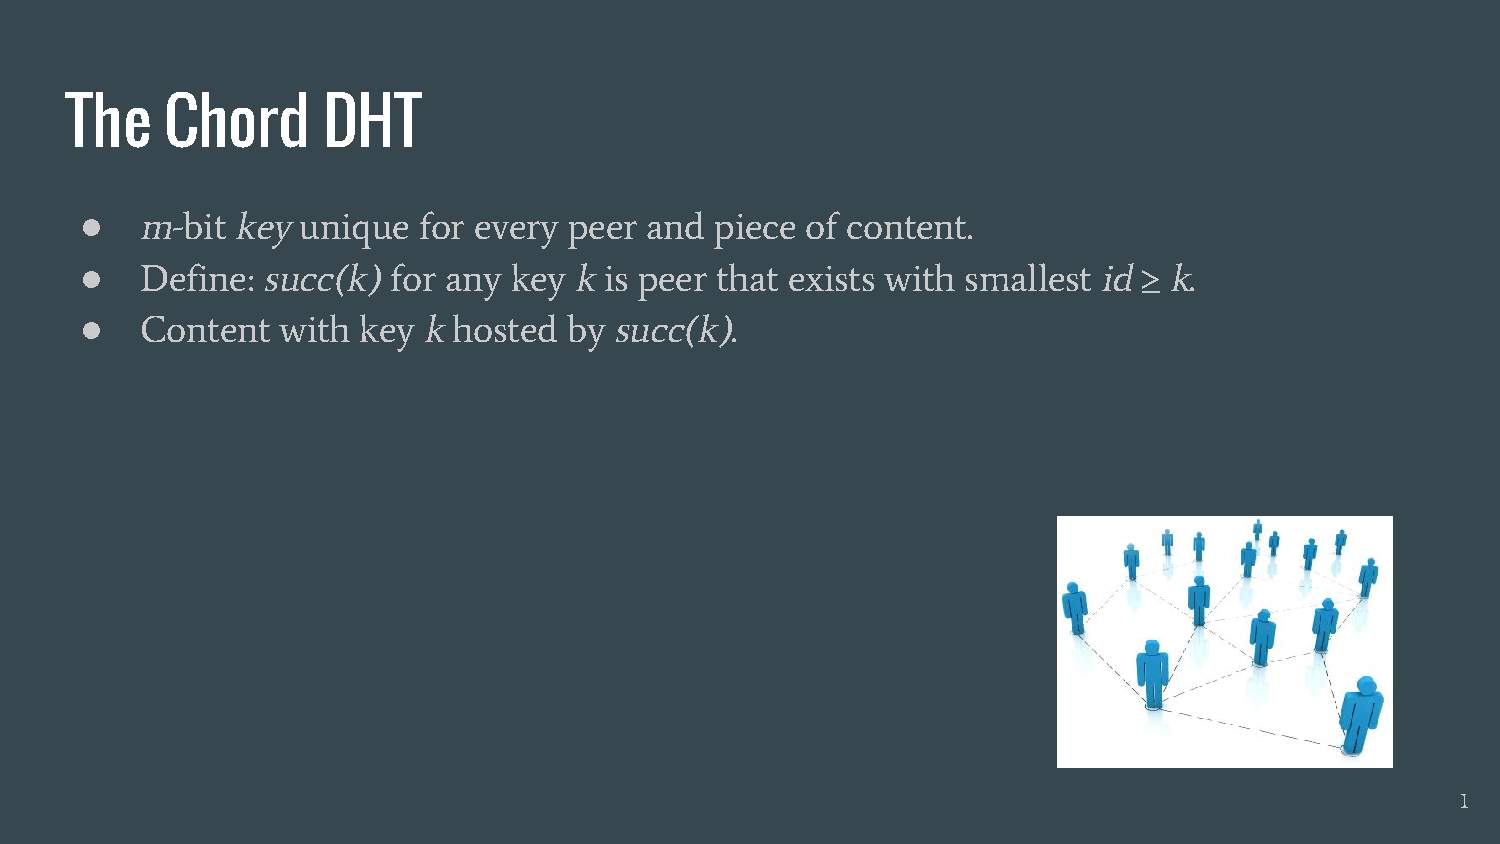
\includepdf[page=1-2]{slides-2.pdf}
We can look at this as a circle. The number of entites that this id space supports is $2^M$. This represents a peer to peer network, each node that we see is a peer on the network. We try to use cord to let people look up peers when they only know the id of one in the network but not the one they are looking for. We care about minimizing the number of hops between peers to get to our requested one. Everytime you hop we decrease a packet's time to live value by one. If it drops to 0 the packet is dropped. We do this so that a bug doesn't lead to packets living forever. The diameter of this graph is the longest distance of the shortest path. We assume that a packet will follow the route that is most optimal (routing protocols try to make the routing tables use only these shortest paths). We look at the internet's diameter as described above, this value must fit within the time to live value of a packet (which is confined to 8 bits). 

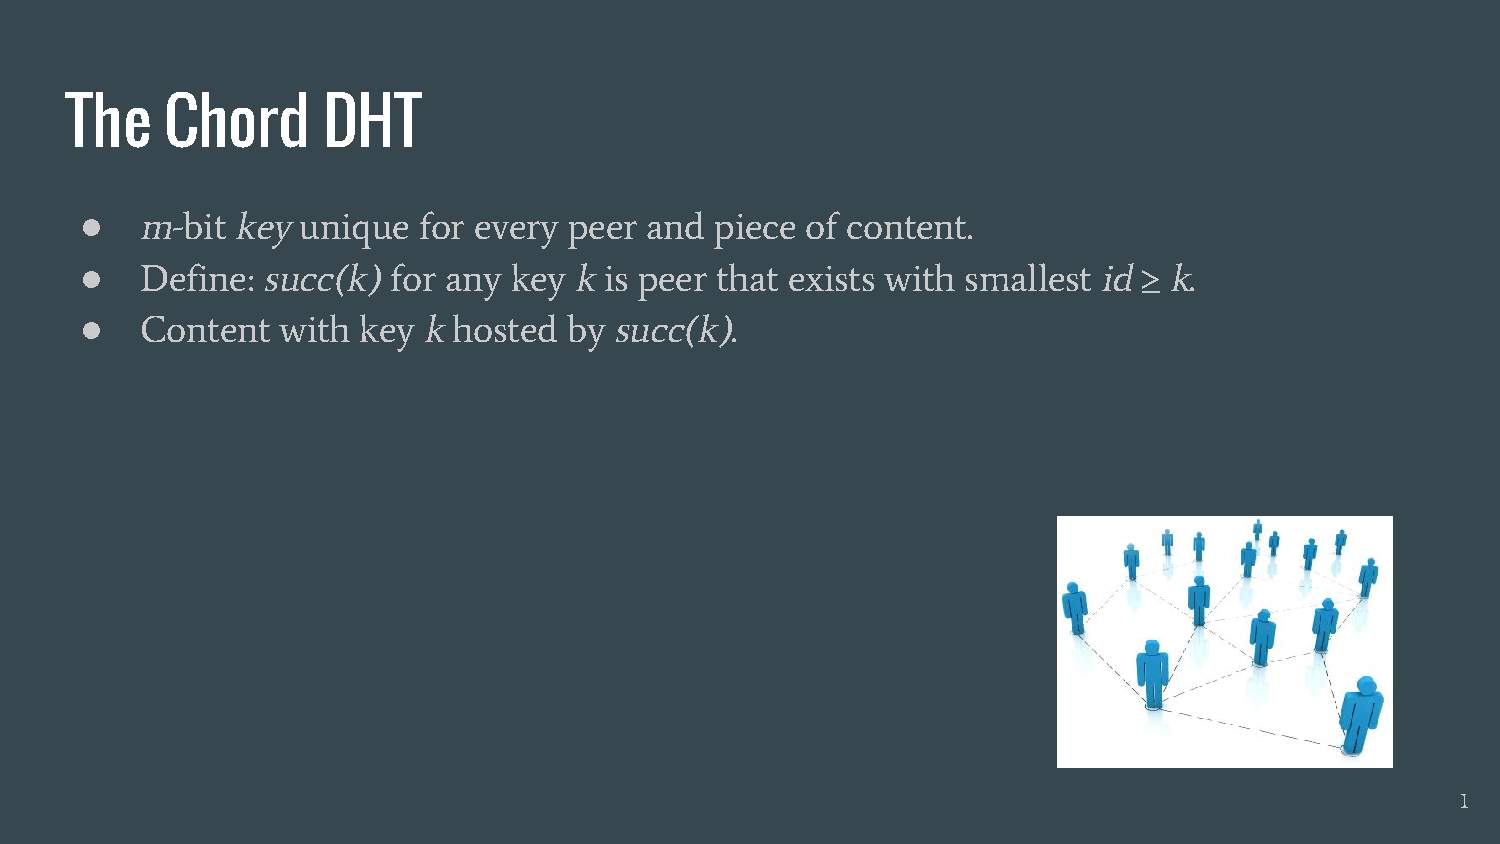
\includepdf[page=3-5]{slides-2.pdf}
We want to use this chord diagram to get the fastest and most space efficient algorithm. We apply that formula to a couple of values (up to m) counting up and figuring out the successor if we were too look for that at each. The worst case space space complexity of this is $m^2$ (so is the average space). If we have an outside client look up peer 12 at peer 28 (ie they only had the address of peer 28 but wanted peer 12). We look at the entries to the table with the greatest number less than 12, at 28 this is 4 so we go to 4. At 4 we do the same thing and go to so on until we get to peer 14 where there is no value less than 12 so this is the correct value. We see in the other example that the last node is still less than the value we are looking for so we hop to the first value in the table of 28. Only a peer of value greater than 12 can host 12 because of how we defined successors (they must have id greater). The successor rule can be broken if there is no other key that works, else it can loop around.

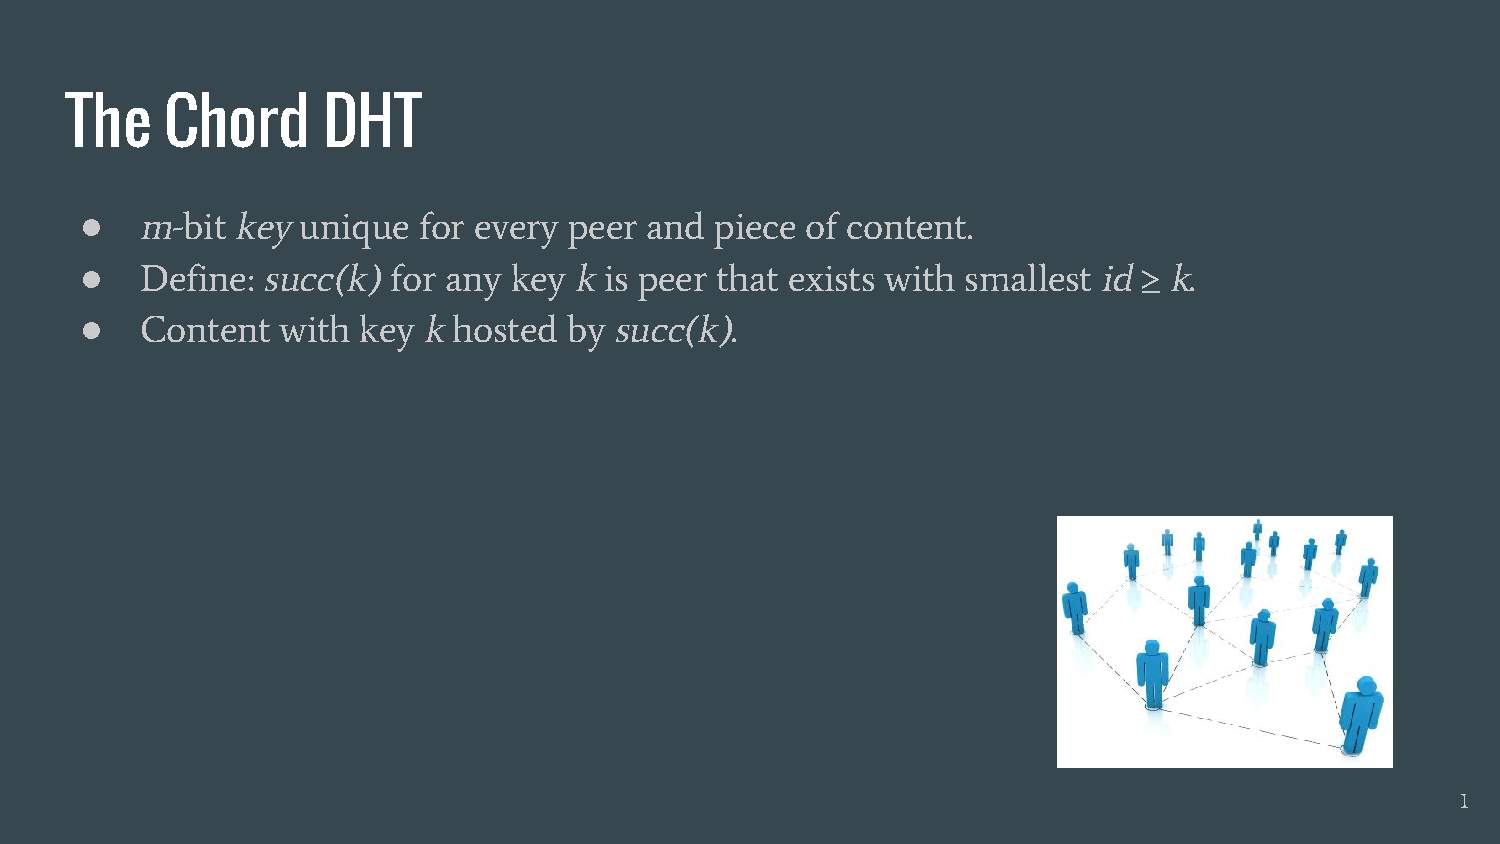
\includepdf[page=6]{slides-2.pdf}
n is the number of peers. This means that the expected number of hops is $O(\log n$. We know that each hop covers half the arc-length (we can see that in a finger table shits grows exponentially making it cover more). When we add a peer we just chose a random number (doing it over again if a collision occurs). 

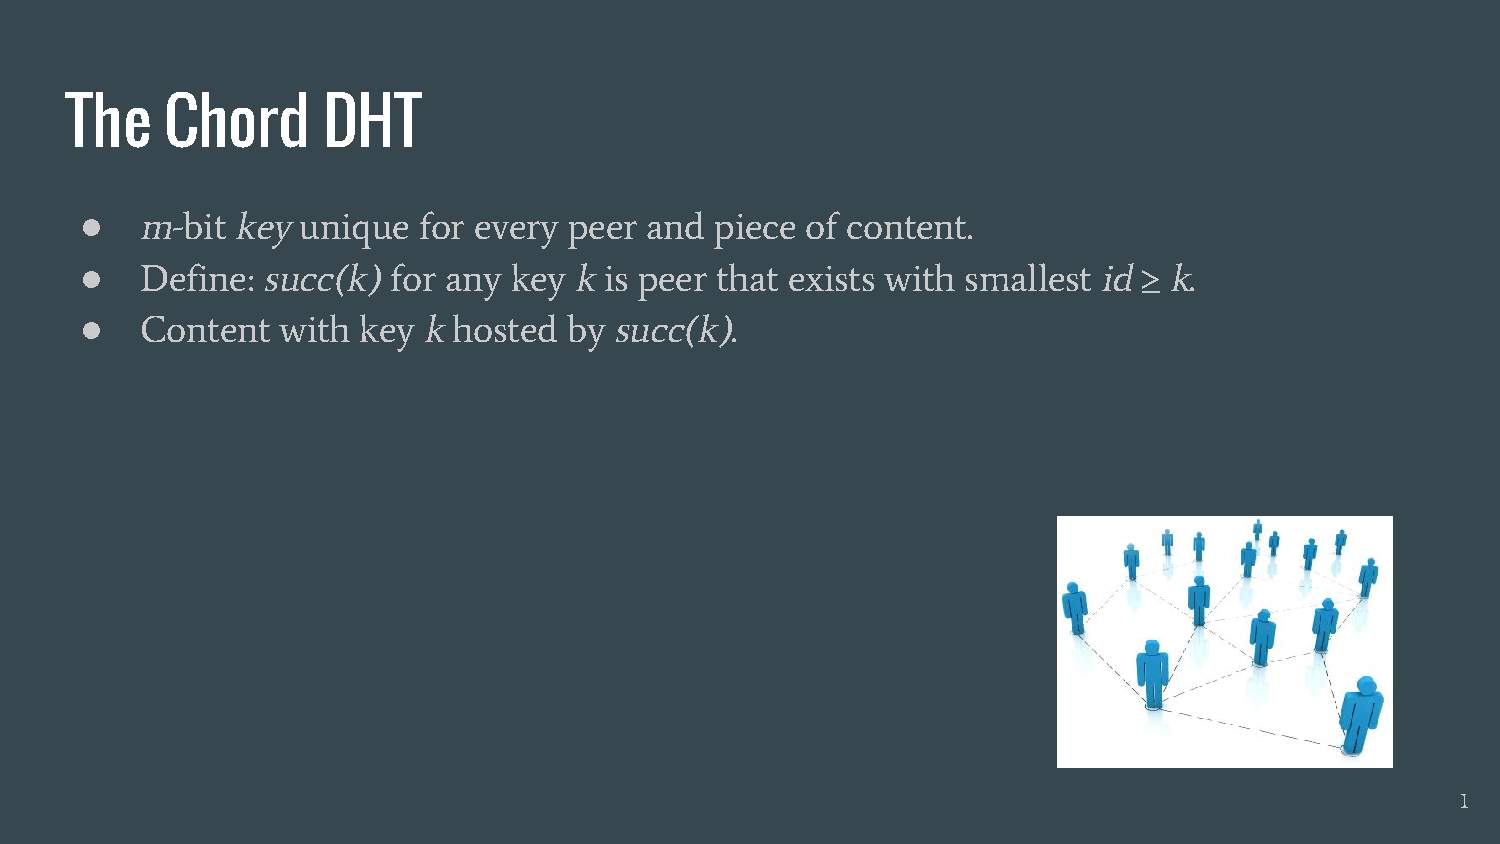
\includepdf[page=7-8]{slides-2.pdf}
when we do a loop up  at q we get that its at the jth entry in the table. So then $q \ge p + 2^{j-1}$ by using our formula for building the table and the definiton of successor. If we say r is the penultimate hop so we know that $r < p + 2^j$ if r was greater than that we would have jumped farther. 

\end{document}